\documentclass[11pt]{exam}
\usepackage[margin=1in]{geometry}
\pagestyle{plain}
\usepackage{amsmath,amsfonts,amssymb,amsthm,enumerate}
\usepackage{multicol}
\usepackage[]{graphicx}
\usepackage{hyperref}
\usepackage{tikz}

\addtolength{\footskip}{2\baselineskip} % to lower the page numbers
\title{\vspace{-1.25in} Math 115 \\ Worksheet Section 1.3}
\date{}


% \theoremstyle{definition}
% \newtheorem{problem}{Problem}
\renewcommand{\questionlabel}{\textbf{Problem~\thequestion.}}
%\printanswers

\begin{document}
\maketitle
\vspace{-1in}
\begin{questions}
  \question 
  \begin{multicols}{2}
	$$\begin{array}{|c|c|c|c|c|} \hline
            x  & -1 & 0 & 1 & 3 \\ \hline
            f(x)  & 2  & -1 & -2  & 2  \\
            \hline
          \end{array}$$	
	
          Use the graph provided for $f(x)$ to sketch the graph and
          fill in some values of the table for some of the related
          functions below. \\ 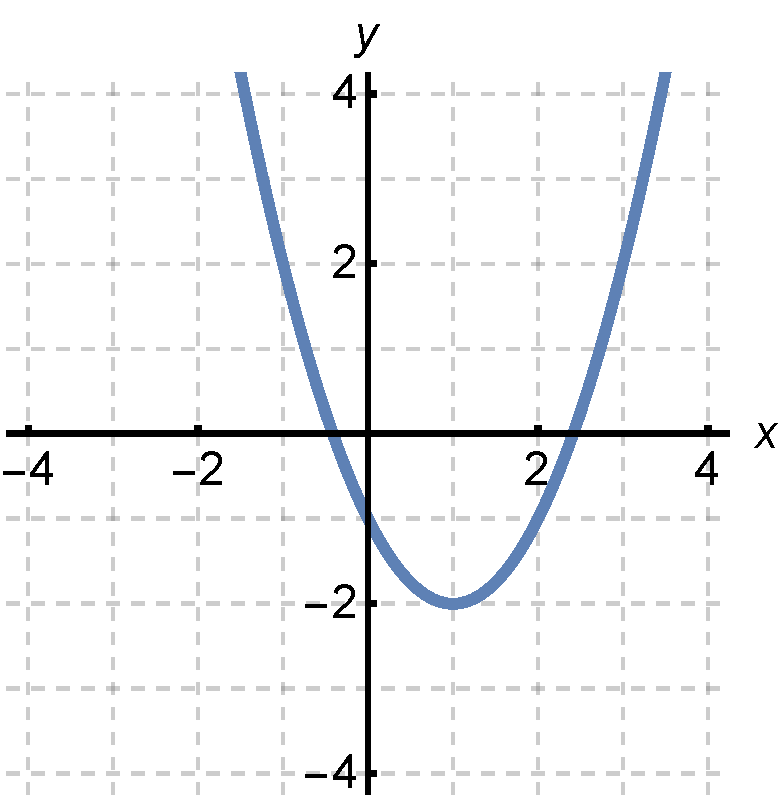
\includegraphics[width=4.5cm]{Figures/parab}
\end{multicols}
\vspace{-0.3in}
\begin{multicols}{2}
 $$\begin{array}{|c|c|c|c|c|} \hline
x  & \hspace{.2in} & \hspace{.2in} & \hspace{.2in} & \hspace{.2in} \\ \hline
f(x)-2 &   &  &  &   \\
\hline
\end{array}$$  \\
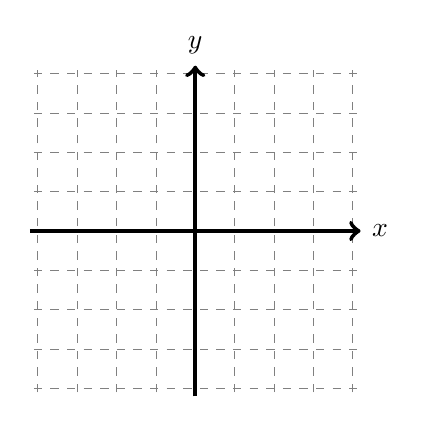
\begin{tikzpicture}[scale=0.5]
\draw[help lines, color=gray, dashed] (-4.1,-4.1) grid (4.1,4.1);
\draw[->,ultra thick] (-4.2,0)--(4.2,0) node[right]{$x$};
\draw[->,ultra thick] (0,-4.2)--(0,4.2) node[above]{$y$};
\end{tikzpicture}

\end{multicols}
\vspace{-0.3in}
\begin{multicols}{2}
 $$\begin{array}{|c|c|c|c|c|} \hline
x  & \hspace{.2in} & \hspace{.2in} & \hspace{.2in} & \hspace{.2in} \\ \hline
f(x-2) &   &  &  &   \\
\hline
\end{array}$$  \\
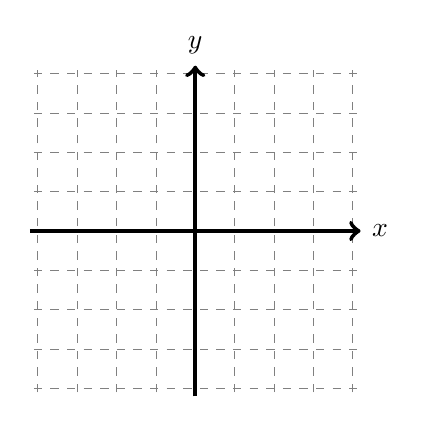
\begin{tikzpicture}[scale=0.5]
\draw[help lines, color=gray, dashed] (-4.1,-4.1) grid (4.1,4.1);
\draw[->,ultra thick] (-4.2,0)--(4.2,0) node[right]{$x$};
\draw[->,ultra thick] (0,-4.2)--(0,4.2) node[above]{$y$};
\end{tikzpicture}

\end{multicols}
\vspace{-0.3in}
\begin{multicols}{2}
 $$\begin{array}{|c|c|c|c|c|} \hline
x  & \hspace{.2in} & \hspace{.2in} & \hspace{.2in} & \hspace{.2in} \\ \hline
-2f(x) &   &  &  &   \\
\hline
\end{array}$$  \\
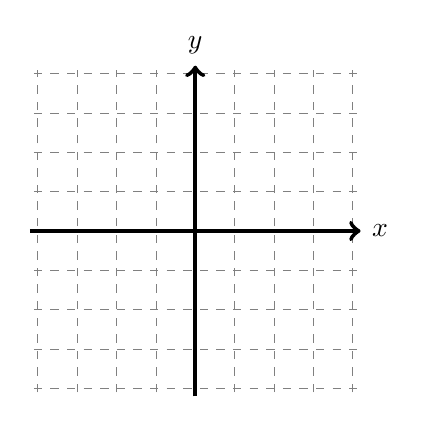
\begin{tikzpicture}[scale=0.5]
\draw[help lines, color=gray, dashed] (-4.1,-4.1) grid (4.1,4.1);
\draw[->,ultra thick] (-4.2,0)--(4.2,0) node[right]{$x$};
\draw[->,ultra thick] (0,-4.2)--(0,4.2) node[above]{$y$};
\end{tikzpicture}

\end{multicols}
\vspace{-0.25in}
\begin{minipage}{0.45\linewidth}
  Consider $f(x)$ above.  First, shift left by 3, then make the graph
  wider by a factor of 2.  Sketch this function, and write down a
  formula for it in terms of $f$.  \vskip2ex Now, start again, but
  this time, first make the graph wider by a factor of 2, then shift
  left by 3.  Again, sketch it and find a formula.  Is it the same
  function that you got previously?
\end{minipage}
\hfill
\begin{minipage}{0.45\linewidth}
  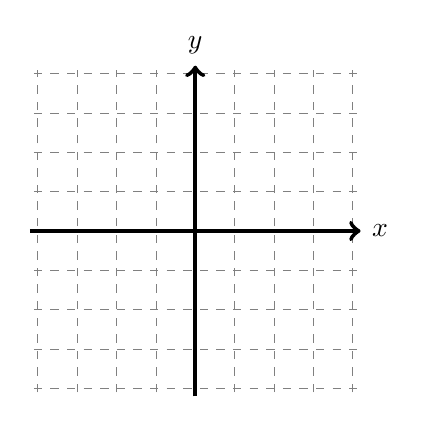
\begin{tikzpicture}[scale=0.5]
    \draw[help lines, color=gray, dashed] (-4.1,-4.1) grid
    (4.1,4.1); \draw[->,ultra thick] (-4.2,0)--(4.2,0)
    node[right]{$x$}; \draw[->,ultra thick] (0,-4.2)--(0,4.2)
    node[above]{$y$};
  \end{tikzpicture}
\end{minipage}
% Verbal description: This is the u
\question
\begin{parts}
	\part For the following graph, estimate $f^{-1}(0)$ and $f^{-1}(2)$, and sketch $f^{-1}$.
	

	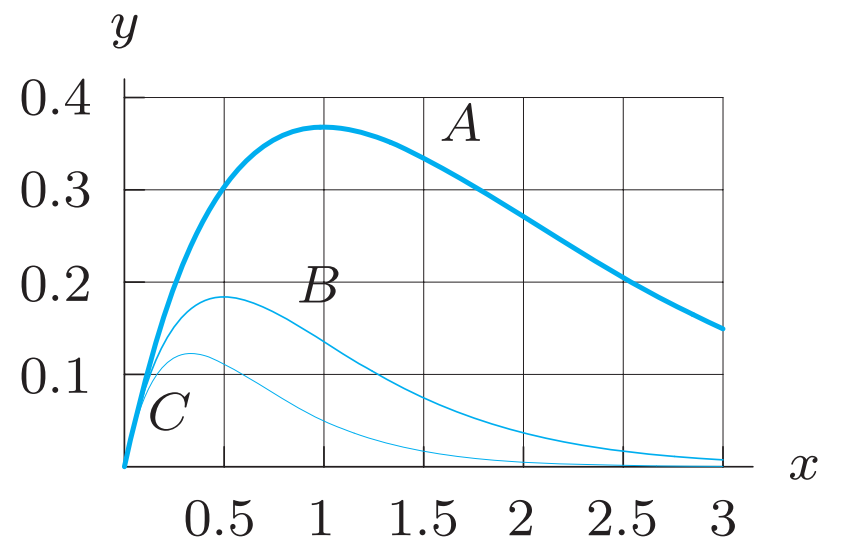
\includegraphics[width=3in]{Figures/graph.jpg}
        \begin{solution}
         \(f^{-1}(0) \approx -2, f^{-1}(2) \approx -1\) 
        \end{solution}
	\part For the following table, find $f(2)$, $f^{-1}(2)$ and $f^{-1}(4)$.
	
	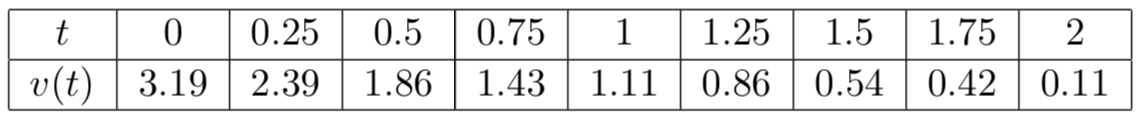
\includegraphics[width=3in]{Figures/table.jpg}
        \begin{solution}
          \(f(2) = -7, f^{-1}(2) = 6, f^{-1}(4) = 4\).
        \end{solution}
	\part Sketch graphs for the heights of a skydiver and a bungee jumper respectively.  Are they invertible?
        \begin{solution}
          The graph of the skydiver is invertible. The graph of the
          bungee jumper is not since a bungee jumper achieves the same
          height at two different times.
        \end{solution}
	\vskip15ex
	\part A function has an inverse if and only if:
	\vskip5ex 
        \begin{solution}
          A function has an inverse if and only if its graph
          intersects any horizontal line at most once. (See p. 27 of textbook.)
        \end{solution}
	
	\part Is $y=f(x) = 3x-5$ invertible?  If so, find the inverse.
        \begin{solution}
          Yes. We see \[
            y = 3x-5 \implies y-5 = 3x \implies x = \frac{y-5}{3}
          \]
        \end{solution}
	
	
	\part (1.3 \#19)
	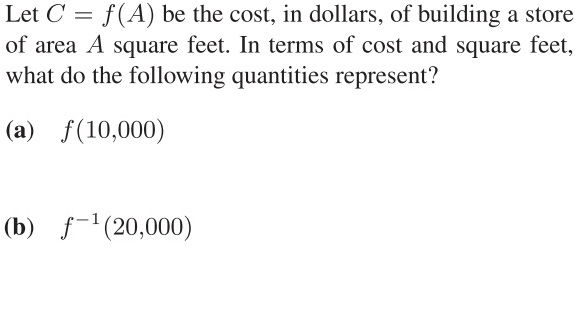
\includegraphics[width=3.5in]{Figures/no19.jpg}
        \begin{solution}
          (a) represents the cost of building a \(10,000\) square foot
          store.\\
          (b) represents the area of a store that costs \(\$20,000\).
        \end{solution}
	\textbf{Function Composition}
	\part (1.3 \#9) Let $f(x) = \sqrt{x+4}$ and $g(x) = x^2$.  Find 	$f(g(x))$ and 
	$g(f(x))$.
        \begin{solution}
          \[
            f(g(x)) = \sqrt{g(x)+4} = \sqrt{x^2+4}
          \]
          \[
            g(f(x)) = (f(x))^2 =(\sqrt{x+4})^2
          \]
        \end{solution}
	\vskip10ex 
        \pagebreak
	\part (1.3 \#48--51)
	
	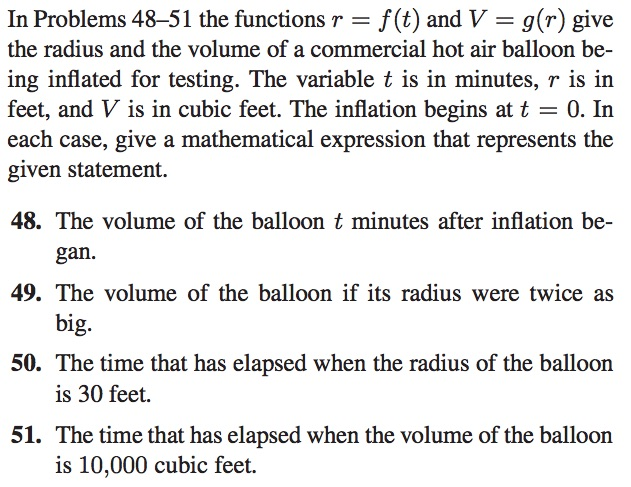
\includegraphics[width=4in]{Figures/no48.jpg}
        \begin{solution}
          \begin{enumerate}
          \item[48.] \(g(f(t))\)
          \item[49.] \(g(2r)\)
          \item[50.] \(f^{-1}(30)\)
          \item[51.] \(f^{-1}(g^{-1}(10000))\)
          \end{enumerate}
        \end{solution}
	\end{parts}
  \question (Fall 2017 Exam 1 Problem 4) The graph of a function
  $Q(x)$ with domain $[-5, 5]$ is shown below.
  \begin{figure}[h]
    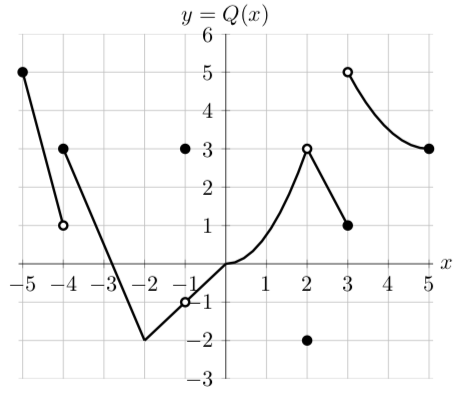
\includegraphics[scale=0.35]{Figures/Graphg}
  \end{figure}
  \begin{parts}
    \part On which of these intervals is $Q$ invertible? Circle
    \underline{all} that are true.
	
	$$[-4, -1] \qquad \qquad [-2,3] \qquad \qquad [2,5] \qquad \qquad [-2,2] \qquad \qquad \textrm{None of these.}$$
	\part For which values of $-5 < x < 5$ is the function $Q$ not
        continuous?
      \end{parts}
      \begin{solution}
        See \href{https://dhsp.math.lsa.umich.edu/exams/115exam1/f17/s4.pdf}{https://dhsp.math.lsa.umich.edu/exams/115exam1/f17/s4.pdf}
      \end{solution}
      \vspace{0.5in}
      \pagebreak
    \question (Winter 2018 Exam 1 Problem 2)
A group of divers recently discovered one of the most submerged caverns in the world. As part of the exploration team, Elena descended into the caverns to take measurements of the temperature and pressure at different depths in the water. Elena started her descent at 8 am and reached the bottom of the caverns at 8:30 am. Let
\vspace{-.05in}
\begin{itemize}
\item $A(t)$ be Elena's depth (in meters) during her descent t minutes after 8 am,
\item $B(p)$ be the depth (in meters) at which Elena measures a water pressure of p kPa
(kiloPascals),
\item C(m) be the water temperature (in degrees Celsius) at a depth of m meters.
\end{itemize}
\vspace{-.05in}
Assume all these functions are invertible.
\begin{parts}
\part Find mathematical expressions that represent each of the sentences below.
\begin{subparts}
\subpart The temperature of the water in degrees Celsius when its pressure is 118 kPa.
\subpart The water pressure, in Pascals, 2 meters under the water surface (1 kPa =1000 Pascals).
\end{subparts}
\vspace{0.5in}
\part At 8:02am, Elena started recording all the data that she was measuring. Let $F(x)$ be Elena's depth (in meters) $x$ seconds after she started recording data. Find a formula for $F(x)$ in terms of any of the functions A, B or C.
  \end{parts}
  \begin{solution}
    See \href{https://dhsp.math.lsa.umich.edu/exams/115exam1/w18/s2.pdf}{https://dhsp.math.lsa.umich.edu/exams/115exam1/w18/s2.pdf}
  \end{solution}
  \question 
Consider the graph of the function $m$ below.
\begin{figure}[h]
\centering
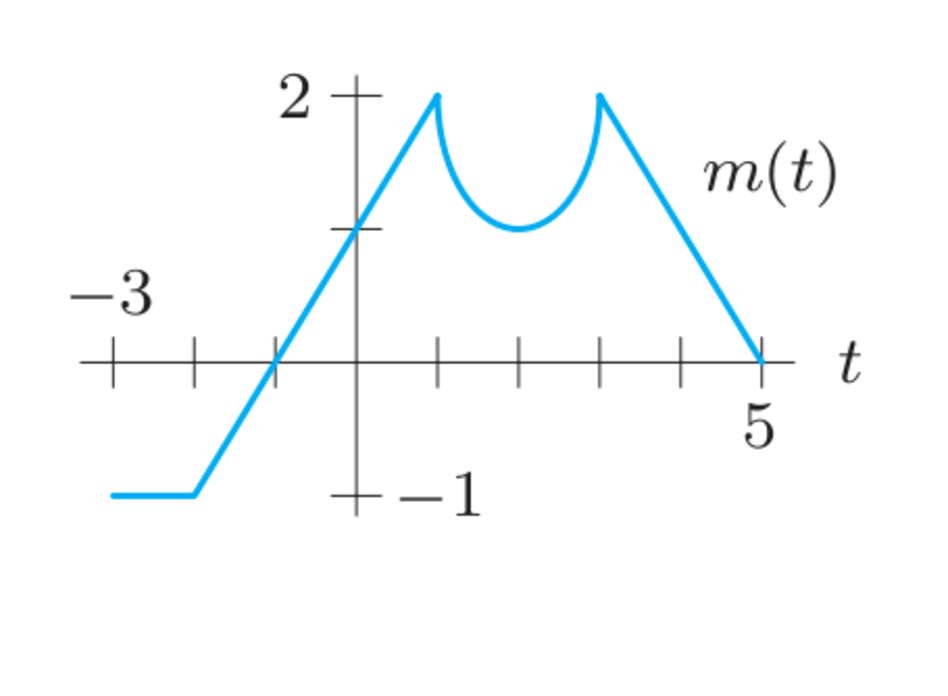
\includegraphics[scale=0.5]{Figures/fig1.pdf}
\caption{Graph of $m$}
\end{figure}
\begin{enumerate}[(a)]

\item What is the domain of $m$?

\item What is the range of $m$?

\item On which interval(s) is the function constant?

\item On which interval(s) is the function linear?

\item On which interval(s) is the function increasing?

\item On which interval(s) is the function decreasing?

\item Graph the following functions:
\[
\text{(i) } n(t) = m(t)+2, \quad \text{(ii) } k(t)= m(t+1), \quad \text{(iii) } z(t) = 2m(t) - 2
\]
\end{enumerate}
\begin{solution}
  \begin{enumerate}[(a)]
  \item The domain is \([-3,5]\).
  \item The range is \([-1,2]\).
  \item The function is constant on \([-3,-2]\).
  \item The function is linear on \([-3,-2], [-2,1]\), and \([3,5]\).
  \item The function is increasing on \([-2,1]\) and \([2,3]\).
  \item The function is decreasing on \([1,2]\) and \([3,5]\).
  \item 
    \vspace{5in}
  \end{enumerate}
\end{solution}
    \end{questions}
  \end{document}
%%% Local Variables:
%%% mode: latex
%%% TeX-master: t
%%% End:
